\chapter[Embasamento Teórico]{Embasamento Teórico}
\label{ch:cap2}
\section[\textit{Contextualizacao}]{\textit{Contextualização}}\label{context}
O Consumo de energia elétrica é um dos principais indicadores de desenvolvimento e de qualidade de vida 
de um país. Esse índice é tão importate que reflete diretamente no rítimo de vida de uma populção, pois mostra
se as atividades industriais de uma nação está ou não em um bom rítimo e pode detectar se o comércio está em alta,
devido aos bens e serviços que o povo adiquiriu. Porém um crescimento desordenado na população e um crescimento
exponencial no consumo de enérgia pode acarretar em problemas para um determinado país.
Analisando os dados \cite{epe-balanco-final}, o consumo de energia
elétrica no Brasil vem crescendo ao longo dos anos, o brasileiro vem consumindo mais energia elétrica, nos últimos
35 anos teve um crescimento médio de 6,72\% dessa demanda, após a crise que o Brasil sofreu entre os anos 2002 e 2005 houve um crescimento
de 4,91\% na demanda energética do país. A \autoref{fig:consumo_energia_total} nos mostra bem o cenário de crise energética que o Brasil vinha
passando ao longo dos anos, até 2008 o país consumia mais do que produzia.

\begin{figure}[h!]
	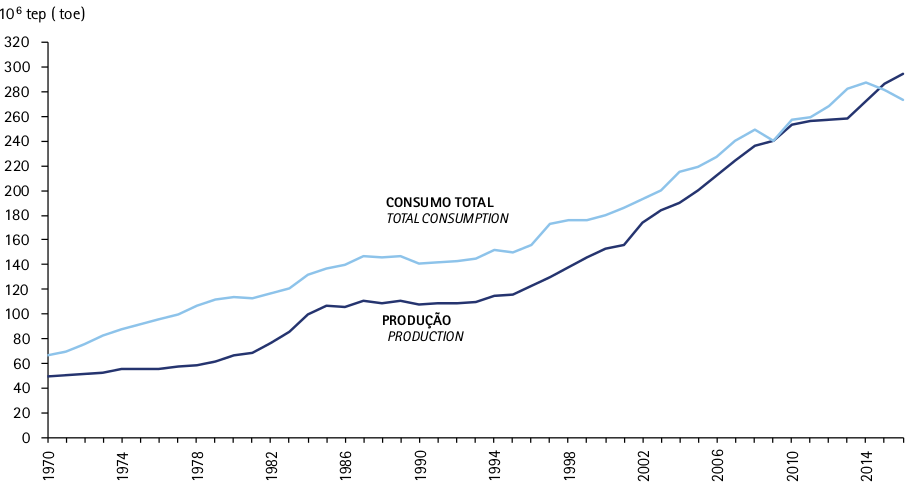
\includegraphics[width=0.85\textwidth, keepaspectratio=true]{consumo_energia_total}
	\centering
	\caption[Estrutura do Consumo de fontes primárias]{Estrutura do Consumo de fontes primárias}
	\fonte{\cite[p. 43]{epe-balanco-final}.}
	\label{fig:consumo_energia_total}
\end{figure}
\FloatBarrier

O governo brasileiro tomou algumas medidas estratégicas para poder acompanhar a crescente demanda por energia elétrica, constituiu o planejamento
da construção de mais de 80 usinas até 2020, hidroelétricas, temoelétricas e até usina nuclear. Um grande problema desse planjamento que o gorverno
fez são os inumeros impactos ambientais e econômicos, um exemplo prático é a usina de de Belo Monte - Rio Xingu, Pará - obra que foi planejada
para ser a quarta maior hidroelétrica do mundo, a maior do Brasil, com capacidade habastecer 40\% das recidências, foi orçada em R\$ 30 bilhões
deveria ter seu início de operação no segundo semestre de 2015 mas até os dias atuais não entrou em funcionamento. Vale salientar que a construção
trouxe o desmatamento de áreas indígenas, alagamentos permanentes, comprometimento da fauna e flora e aumento da dificuldade dos transportes fluviais
de comunidades ribeirinhas.

Analisando a grande demanda energetica que o brasileiro vem requerindo e levando em conta as consquências negativas do planejamento das 80 usinas,
surgi uma questão bastante recorrente: - "O que fazer? Constuir usinas mesmo sabendo dos impactos negativos que podem surgir, ou não construí-las e
aumentar a tarifação pelo consumo de energia visando diminuir o consumo?" - A resposta para essas e outras questões que podem aparecer não são fáceis.
Entretanto o governo brasileiro optou por deixar o consumo de energia elétrica mais caro, principalmente nos horários de pico. A evolução da tarifa,
pode ser observada na \autoref{evolucao-tarifa}


\begin{table}[!ht]
	\centering
	\begin{tabular}{lcccc}
	\hline
	\textbf{Ano} & \multicolumn{1}{l}{\textbf{1º Trimestre}} & \multicolumn{1}{l}{\textbf{2º Trimestre}} & \multicolumn{1}{l}{\textbf{3º Trimestre}} & \multicolumn{1}{l}{\textbf{4º Trimestre}} \\ \hline
	\rowcolor[HTML]{DDDDDD} 
	2013         & 120,8                                     & 117,1                                     & 114,5                                     & 116,1                                     \\
	2014         & 121,1                                     & 127,6                                     & 134,4                                     & 141,9                                     \\
	\rowcolor[HTML]{DDDDDD} 
	2015         & 154,2                                     & -                                         & -                                         & -                                        
	\end{tabular}
	\caption{Evoluçao dos custos de energia elétrica em R\$/MWh}
	\fonte{\cite[p. 1]{evolucao-tarifa-ref}}
	\label{evolucao-tarifa}
\end{table}

Uma medida totalmente cabível que ainda é desconhecida por alguns brasileiros é a chamada "\textit{exposição da informação}", deixando sempre bem claro 
quanto o consumidor tem gastado ou consumindo ao longo do mês em sua recidência, isso é possível graças a equipamentos que estão sempre monitorando
a rede elétrica.Segundo uma pesquisa realizada pela Associação Brasileira das Empresas de Serviços de Conservação de Energia, seis anos o Brasil 
desperdiçou o equivalente a 250GWh em energia o que equivale a R\$62 bilhões, desperdíciu que se deu justamente a tamanha falta de infomação que 
o consumidor tem, se ao saber o quanto tem consumido ou gastado em tempo real o consumidor poderia se prevenir dos desperdícios. 

\subsection[\textit{Setor Energético Brasileiro}]{\textit{Setor Energético Brasileiro}}\label{seb}
Ao passar dos anos o Brasil vem mostrando cada vez mais o seu potencial na produão de energia, o território brasileiro possibilita as várias formas
de obtenção da eletricidade. Analisando os dados \cite[p.29]{epe-anuario-2015} e comparando com a \autoref{cap_ele} nota-se que o Brasil subiu duas
posoções no \textit{Rank} de geração de energia elétrica, isso é reflexo do aumentou da capicidade de produção de energia que chegou na marca de 8,39\%.

\begin{table}[!ht]
	\centering
	\begin{tabular}{lccccc}
		\rowcolor[HTML]{9B9B9B} 
		\multicolumn{1}{c}{\cellcolor[HTML]{9B9B9B}} & {\color[HTML]{FFFFFF} \textbf{2010}} & {\color[HTML]{FFFFFF} \textbf{2011}} & {\color[HTML]{FFFFFF} \textbf{2012}} & {\color[HTML]{FFFFFF} \textbf{2013}} & \multicolumn{1}{l}{\cellcolor[HTML]{9B9B9B}{\color[HTML]{FFFFFF} \textbf{2014}}} \\ \hline
		\textbf{Mundo}                               & \multicolumn{1}{l}{\textbf{5080,6}}  & \multicolumn{1}{l}{\textbf{5305,0}}  & \multicolumn{1}{l}{\textbf{5514,6}}  & \multicolumn{1}{l}{\textbf{5736,2}}  & \multicolumn{1}{l}{\textbf{6038,7}}                                              \\ \hline
		\rowcolor[HTML]{DDDDDD} 
		China                                        & 971,8                                & 1069,5                               & 1154,6                               & 1267,7                               & 1399,5                                                                           \\
		Estados Unidos                               & 1039,1                               & 1051,3                               & 1063,0                               & 1060,1                               & 1074,6                                                                           \\
		\rowcolor[HTML]{DDDDDD} 
		Japão                                        & 284,9                                & 287,3                                & 293,3                                & 300,8                                & 313,4                                                                            \\
		Índia                                        & 213,1                                & 246,0                                & 260,3                                & 283,0                                & 310,8                                                                            \\
		\rowcolor[HTML]{DDDDDD} 
		Rússia                                       & 228,1                                & 231,6                                & 233,6                                & 235,2                                & 247,6                                                                            \\
		Alemanha                                     & 162,7                                & 167,5                                & 177,3                                & 186,1                                & 198,4                                                                            \\
		\rowcolor[HTML]{DDDDDD} 
		Canadá                                       & 132,3                                & 132,9                                & 130,7                                & 133,3                                & 136,8                                                                            \\
		Brasil                                       & 11,3                                 & 117,1                                & 121,0                                & 126,7                                & 133,9                                                                           
	\end{tabular}
	\caption{Capacidade instalada de geração elétrica no mundo, 2014 (GW)}
	\fonte{\cite[p. 29]{epe-anuario}}
	\label{cap_ele}
\end{table}

A maior produção de energia do Brasil provem das hidroelétricas, o país é referência mundial quando o assunto é obtenção de energia através de
usinas hidroelétricas - \autoref{cap_hidro} - isso é possível devido a sua alta concentração de rios de grande porte e ao grande volume de chuva
que alimenta e reforça o poderio hídrico do país. A energia que a usina hidroelétrica fornece é conseguida através da energia hidráulica que provém
do aproveitamento da força potencial e cinética das correntes de água,rio, mar. A água ao passar por tubulações com muita força e velociadade 
movimentas as turbinas fazendo com que elas girem em um velociadade suficiente para que os geradores acoplados nas turbinas, transformem energia
mecânica em energia elétrica, lembrando que a eficiência energética de uma usina hidroelétrica é de 65,2\%. Após esse longo processo a energia 
extraída é enviada para estações de tratamento onde e após isso é enviada para a matriz energetica que fará a distribuião da energia extraída. 

\begin{table}[!ht]
	\centering
	\begin{tabular}{lccccl}
		\rowcolor[HTML]{9B9B9B} 
		\multicolumn{1}{c}{\cellcolor[HTML]{9B9B9B}} & {\color[HTML]{FFFFFF} \textbf{2010}} & {\color[HTML]{FFFFFF} \textbf{2011}} & {\color[HTML]{FFFFFF} \textbf{2012}} & {\color[HTML]{FFFFFF} \textbf{2013}} & {\color[HTML]{FFFFFF} \textbf{2014}} \\ \hline
		\textbf{Mundo}                               & \multicolumn{1}{l}{\textbf{903,9}}   & \multicolumn{1}{l}{\textbf{929,9}}   & \multicolumn{1}{l}{\textbf{957,5}}   & \multicolumn{1}{l}{\textbf{1000,4}}  & \textbf{1038,3}                      \\ \hline
		\rowcolor[HTML]{DDDDDD} 
		China                                        & 199,5                                & 214,6                                & 229,1                                & 258,9                                & 283,0                                \\
		Brasil                                       & 80,7                                 & 82,5                                 & 84,3                                 & 86,0                                 & 89,2                                 \\
		\rowcolor[HTML]{DDDDDD} 
		Estados Unidos                               & 78,8                                 & 78,7                                 & 78,7                                 & 79,2                                 & 79,7                                 \\
		Canadá                                       & \multicolumn{1}{l}{74,9}             & \multicolumn{1}{l}{75,4}             & \multicolumn{1}{l}{75,4}             & \multicolumn{1}{l}{75,4}             & 75,4                                
	\end{tabular}
	\caption{Capacidade instalada de geração hidrelétrica no mundo, 2014 (GW)}
	\fonte{\cite[p. 30]{epe-anuario}}
	\label{cap_hidro}
\end{table}

Como já mencionado nesse trabalho o Brasil possui um vasto território, possibilitando inúmeras formas para obtenção de energia. 

\begin{table}[!ht]
	\centering
	\begin{tabular}{cccc}
		\hline
	\textbf{Região} & \textbf{População} & \textbf{Consumo em GW} & \textbf{\begin{tabular}[c]{@{}c@{}}Capacidade Instalada de \\ Geração Elétrica GW\end{tabular}} \\ \hline
		\rowcolor[HTML]{DDDDDD} 
		Norte           & 17.707.783         & 12.197                 & 25,484                                                                                          \\
		Nordeste        & 56.915.936         & 12.109                 & 29,803                                                                                          \\
		\rowcolor[HTML]{DDDDDD} 
		Sudeste         & 86.356.952         & 74.584                 & 44,810                                                                                          \\
		Sul             & 29.439.773         & 19.173                 & 31,681                                                                                          \\
		\rowcolor[HTML]{DDDDDD} 
		Centro-Oeste    & 15.660.988         & 5.634                  & 18,558                                                                                         
	\end{tabular}
	\caption{Relação Populaão x Consumo por Região x Geração Elétrica por Região}
	\fonte{(IBGE e EPE)}
	\label{pxcxge}
\end{table}
